\section{直接対決}
時は来た。後の伝説となった直接対決の模様を解説していく。

\subsection{ライブという概念}
上記の通り、とうとう我々は、クボタアツム要する藤岡弘、との試合を行うこととなった。試合は順調に進んでおり、我々は、試合会場の後方側で来るべきときに備えて虎視眈々と、クボタアツムと大魔神の一致に対する5$\sigma$の可能性を探っていた。
試合の構成は、上記でも述べた通り、なんかしょうもない曲披露が中心であり、その後、握手券を持つ者や、チェキ券を持つ者という選ばれし重症患者のみが次のステージに上がれるという、極めて厳しい戦いである。試合自体は順調に進み、いよいよ試合後の握手タイムの雰囲気が漂い始めた頃、ついにあの男が動き出すのである。そう、アツムである。

\subsection{チェキ代は奢る}
ここで時刻はさかのぼり、百年前の出来事である。オガワインティライミ氏が「直接対決をしない限り$5 \sigma$を認めない」と宣言していた頃、水面下でその試合についての交渉が行われていた。交渉内容としては、ただ単に某地下団体の試合のためにわざわざ交通費や観戦料を払いたくないというインティライミ氏側と、預金残高1000万オーダーのATM氏側との対立である。そして、その幾度となく繰り返された激論の末、ATM氏はこう言い放ったのである。\\

\shadowbox{{\Large チェキ代は奢る}}

オガワインティライミは、その一言を全ての原動力として、必死に戦っていたのである。
\subsection{直接対決}
チェキ代(2000円)を奢って貰ったオガワインティライミ氏は、とうとう直接対決をするのである。勝負は一瞬であったが、非常に濃い時間であった。その詳細を述べていく。

\subsubsection{はじめの一歩}
まず、基本的にチェキという制度は、舞台上で待ち構えている藤岡弘、たちに対して、チェキ代を支払った重症患者のみが参列することができる空間に集合し、並ぶ。そしてその列の先頭から順に、チェキという名の試合をしたい人間を宣言し、ばちばちに殴りあうのである。つまり、オガワインティライミ氏もチェキ代を奢って貰ったとはいえ、他のうんこ共と同じようにチェキへの道に並ばなければいけないのである。しかもそれまでは行動を共にしていた学長、先生、ATMとはここでお別れなのである。まさにそこからは、はじめの一歩なのである。

\subsubsection{殴り合い}
チェキロード参列中、あくまで「クボタアツムは大魔神ではない」という主張をしているオガワインティライミ氏は、目と鼻の先に確かに存在するクボタアツムの様子を凝視していた。その時点で、やはり「似ている」と感じるティライミであった。\par
そして、とうとうチェキロードの先頭に立ったオガワインティライミ氏に対し、店員みたいなカスが「どなたにしますか?」と言い放ち、「クボタアツムで」と答えた瞬間から、戦いのゴングが鳴り響いたのである。以下、その一部始終をノーカットでご覧いただく。\\
(オガワインティライミ、登壇)\\
\shadowbox{クボタアツム「選んでくれてありがと〜☆」}\\
\shadowbox{インティライミ「......俺のこと覚えてる?$\sf{ (´\_ゝ`)}$笑」}\\
(インティライミヒント:初対面)\\
\shadowbox{クボタアツム「...え!?オガワくん!??」}\\
\shadowbox{インティライミ「やっぱり大魔神?笑」}\\
\shadowbox{クボタアツム「うわーびっくりしたーー」}\\
\shadowbox{インティライミ「なんか似てるなと思ってたから確かめに来たわ(笑)」}\\
\shadowbox{クボタアツム「すごい!わざわざ!?ありがとー笑」}\\
\shadowbox{インティライミ「一応誰にも言ってないけど知ってる人いるん?」}\\
\shadowbox{クボタアツム「うーん...いないと思うなあ」}\\
\shadowbox{インティライミ「まあせやろな、しかしおもろいな(笑)」}\\
\shadowbox{
\begin{tabular}{l}
スタッフ「それではチェキ撮りまーす、はいチーズ!\\
 \ \ \ \ \ \ \ \ \ \ \ \ \ \ はい、ではクボタアツムちゃんにサインを書いてもらいましょう!」
\end{tabular}}\\
\shadowbox{クボタアツム「はーい!(笑)(クボタアツム、と記入)」}\\
\shadowbox{インティライミ「いや何がクボタアツムや(笑)大魔神やろ(笑)」}\\
\shadowbox{クボタアツム「ちょっと、内緒内緒(笑)」}\\
\shadowbox{スタッフ「はいそれでは、ありがとうございましたー」}\\
\shadowbox{インティライミ「はい、ほな$\sf{ (´\_ゝ`)}$」}\\
\shadowbox{クボタアツム「ありがとー(笑)またねー(笑)」}\\
\shadowbox{インティライミ「なにがありがとーや$\sf{ (´\_ゝ`)}$」}\\
\shadowbox{クボタアツム「ありがとー(笑)」}\\

\subsubsection{余韻}
お分りいただけただろうか。上記の通り、大魔神とオガワインティライミの試合は伝説となったのである。\par
そして、クボタアツムは大魔神だったのである。完全に大魔神だったのである。インティライミは本拠地に戻ったその瞬間、クボタアツム大魔神について、完全に「$5\sigma$」を宣言したのである。とうとう、である。ようやく、である。\par
それからというものの、オガワインティライミにとってその試合会場はもはや大魔神がどういう様子であるかを注視するだけの空間になっていた(図\ref{livekaijo})。\par
一方で、当然チェキの時間はまだ続く。そして、その終了間際は司会がカウントダウンを始めるのだが、本物の重症患者たちが必死に追加で課金して新たにチェキを撮るのである。特に印象的だったのは、ラストスパートのカウントダウン時にある本物の重症患者がチェキを買うためにオガワインティライミの前方を通過した際につぶやいた一言「時間を止める...!」である。キモすぎる上に、時間を止めたところで大魔神にとっては所詮金ヅルの臭いおっさんなのである。もちろん、ATMもその一人である。\par
こうして、試合は終了した。アンコールみたいなのがあり、最後に藤岡弘、たちが全員登壇して観客全員に手を振っていたのだが、オガワインティライミは敢えて会場の前方で手を振ると、大魔神は少々苦笑いをしながらオガワインティライミの方へと手を振ったのである。完全に、$5\sigma$なのである。\par

\begin{figure}[H]
\centering
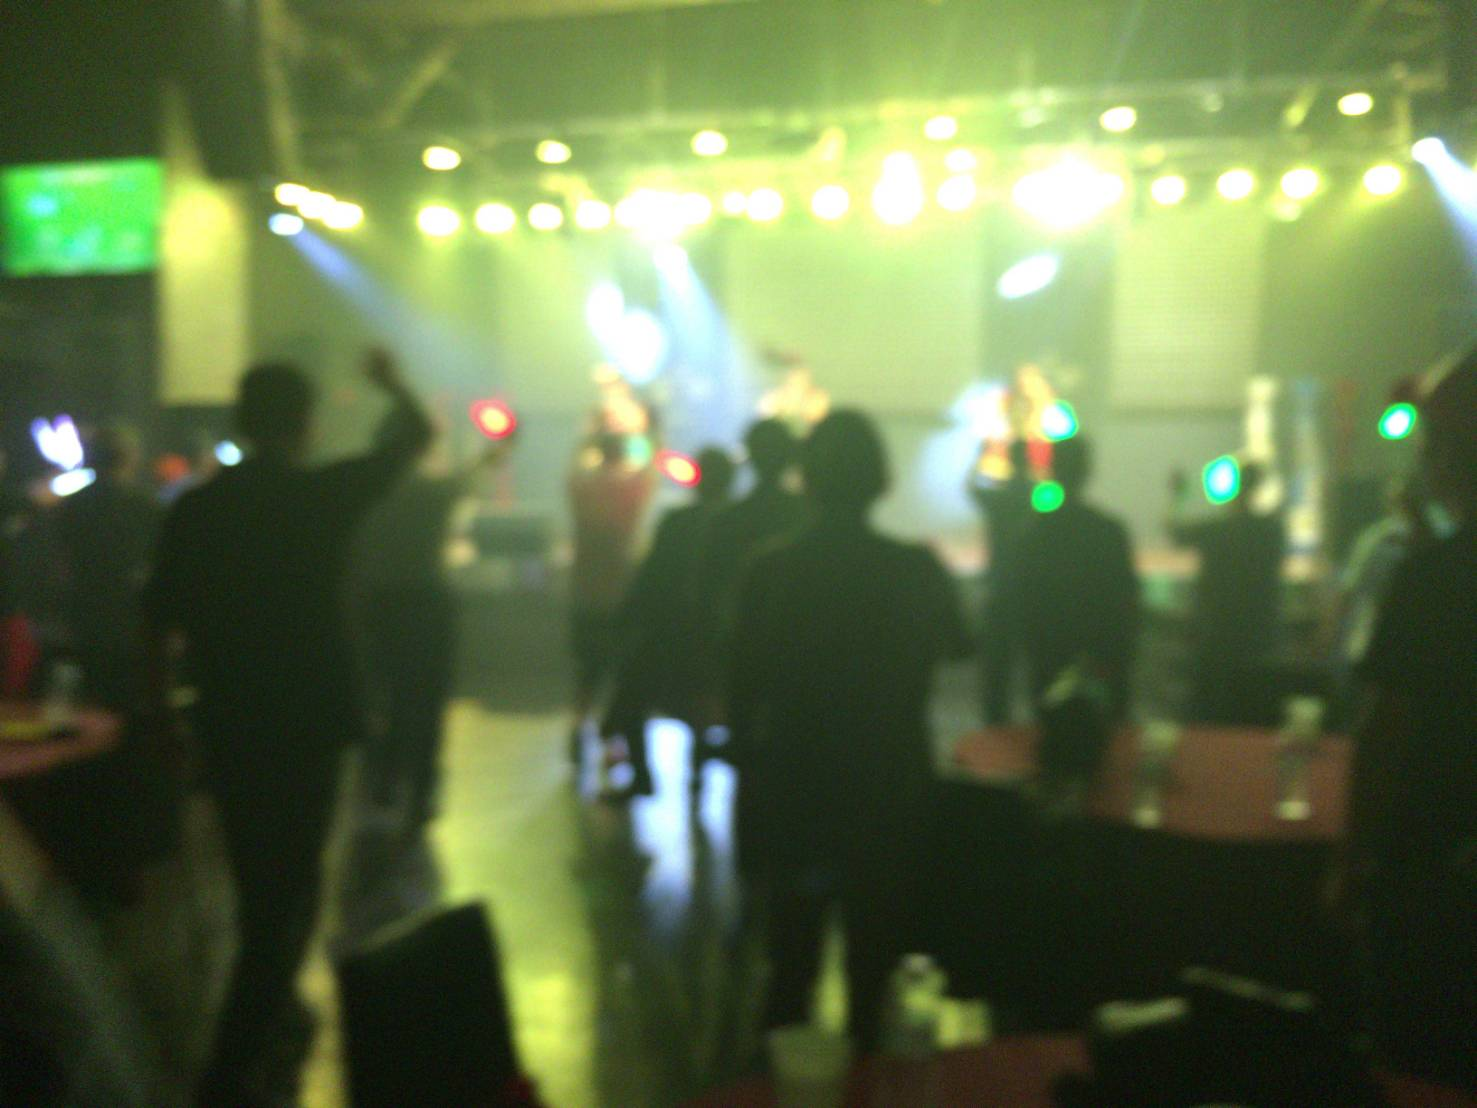
\includegraphics[clip,scale=0.15]{livekaijo.jpg}
    \caption{どう考えても、ここにいた客層は下に見ざるをえない}
    \label{livekaijo}
\end{figure}




